\lecture{10}{2026.05.18}{}

\section{Approximation}

\subsection{Function Approximation}

Given data points $\{(x_i,y_i)\}_{i=1}^n$, we want to find a function $f$ such that \[
    y_i = f(x_i), \quad i=1,2,\dots,n.
\]
However, the data may contain noise, so there is no need to find a function that fits the data points exactly. Instead, we can find a function that approximates the data points well.

The problem becomes minimizing the error \begin{equation}
    E(f) = \min_{f} \sum_{i=1}^n (y_i - f(x_i))^2 \label{eq:1}
\end{equation}
or 
\begin{equation*}
    E(f) = \min_{f} \sum_{i=1}^n |y_i - f(x_i)|
\end{equation*}
with \[
    f(x) = ax + b
\]
\begin{remark}
    We have to make some restrictions on the function $f$ to avoid arbitrary solutions.
\end{remark}
Assume that $x \in \mathbb{R}^1, y \in \mathbb{R}^1$.
\begin{note}
    Square error is more commonly used than absolute error because it is easier to optimize with its differentiability.
\end{note}
Then \ref{eq:1} becomes ``least squares'' problem. 

\subsection{Least Squares Approximation}

\begin{definition}[Least Squares]
    Now the goal becomes to find $a$ and $b$ such that \[
        \min_{a,b} E = \min_{a,b} \sum_{i=1}^n (y_i - (ax_i + b))^2
    \]
\end{definition}
Then we rewrite the objective to let constants in the first term
\begin{eqnarray*}
\min_{a,b}  \sum_{i=1}^n 
(y_i - (ax_i + b))^2
& \equiv & 
\min_{a,b}  \sum_{i=1}^n  y_i^2 - 2y_i
(ax_i+b) + (ax_i + b)^2\\
& \equiv & 
\min_{a,b}  \sum_{i=1}^n   - 2y_i
(ax_i+b) + a^2x^2_i + 2abx_i + b^2 \\
& \equiv & 
\min_{a,b}  \bigg ( (\sum_{i=1}^n -2y_i x_i)a +
( \sum_{i=1}^n - 2y_i)b + 
(\sum_{i=1}^n x_i^2)a^2 + (\sum_{i=1}^n 2x_i)ab + n b^2\bigg )
\end{eqnarray*}

We do the partial derivatives with respect to $a$ and $b$ and set them to zero to find the optimal solution. We have \[
    \frac{\partial E}{\partial a} = \sum_{i=1}^n -2y_i x_i + 2 \left(\sum_{i=1}^n x_i^2\right)a + \left(\sum_{i=1}^n 2x_i\right)b = 0
\]
and \[
    \frac{\partial E}{\partial b} = \sum_{i=1}^n -2y_i + \left(\sum_{i=1}^n 2x_i\right)a + 2nb = 0
\]
We have two equations and two unknowns, so we can solve for $a$ and $b$. Rearranging the equations, we define 
\begin{definition}
    \[
        S_{xx} = \sum_{i=1}^n x_i^2, \quad S_{x} = \sum_{i=1}^n x_i
    \]
    \[
        S_{xy} = \sum_{i=1}^n x_i y_i, \quad S_{y} = \sum_{i=1}^n y_i
    \]
\end{definition}
The equations become \begin{gather*}
S_{xx} a + S_x b = S_{xy}\\
S_x a + n b = S_y 
\end{gather*}
Then solve the problem by Gaussian elimination: \begin{gather*}
a = \frac{n S_{xy} - S_x S_y}{n S_{xx} - S_x^2}\\
b = \frac{S_{xx} S_y - S_x S_{xy}}{nS_{xx} - S_x^2}
\end{gather*}

Now the problem becomes finding that ``Does $\nabla E = 0$ guarantee that we have found the minimum?'' For this problem, we need secondary derivatives (i.e., $\nabla^2 E$) to be positive semi-definite.
\[
    \nabla^2 E = \begin{pmatrix}
        \frac{\partial^2 E}{\partial a^2} & \frac{\partial^2 E}{\partial a \partial b}\\
        \frac{\partial^2 E}{\partial b \partial a} & \frac{\partial^2 E}{\partial b^2}
    \end{pmatrix} = \begin{pmatrix}
        2 S_{xx} & 2 S_x\\
        2 S_x & 2n
    \end{pmatrix}
\]
\begin{note}
    Why semi-definite can guarantee that we have found the minimum? Because if $\nabla^2 E$ is positive semi-definite, then $E$ is convex, and any critical point of a convex function is a global minimum.
\end{note}

We have $S_{xx} \geq 0$ and $n > 0$, and determinant \[
    \det(\nabla^2 E) = S_{xx} n - S_x^2 = \sum_{i=1}^n x_i^2 \sum_{i=1}^n 1 - \left(\sum_{i=1}^n x_i\right)^2 \geq 0
\]
Remember Cauchy-Schwarz inequality: \[
    \left(\sum_{i=1}^n a_i b_i\right)^2 \leq \left(\sum_{i=1}^n a_i^2\right) \left(\sum_{i=1}^n b_i^2\right)
\]
Now consdier an extension ``Nonlinear least squares''
\begin{definition}[Nonlinear least squares]
    Define \[
        E(a,b) = \sum_{i=1}^n (y_i - f(x_i))^2
    \]
    where $f(x) = ax^2 + bx + c$. Then we solve \[
        \min_{f} E = \min_{a,b,c} E(a,b,c)
    \]
\end{definition}
The situation is similar to linear least squares.

\subsection{Higher Dimensional Space}

\begin{definition}
    If $x \in \mathbb{R}^m,\ m > 1$ then \[
        f(x) = a^\top x + b,\ a \in \mathbb{R}^m
    \]
    Let \[
        E = \sum_{i=1}^n (y_i - a^\top x_i - b)^2
    \]
\end{definition}

Then the problem is \begin{equation*}
\begin{split}
\min_{a,b}  \sum_{i=1}^n 
(y_i - (a^\top x_i + b))^2
\equiv &
\min_{a,b}  \sum_{i=1}^n  y_i^2 - 2y_i
(a^T x_i+b) + (a^\top x_i + b)^2\\
\equiv & 
\min_{a,b}  \sum_{i=1}^n   - 2y_i
(a^\top x_i+b) + (a^\top x_i)^2 + 2ba^\top x_i + b^2 \\
\equiv & 
\min_{a,b}  (\sum_{i=1}^n -2y_i x_i)^\top a +
( \sum_{i=1}^n - 2y_i)b + \sum_{i=1}^n (a^\top x_i)^2 + (\sum_{i=1}^n 2x_i)^\top ab + n b^2
\end{split}
\end{equation*}
Then we do the partial derivatives with respect to $a$ and $b$ and set them to zero to find the optimal solution. We have \[
    \frac{\partial E}{\partial a} = \sum_{i=1}^n -2y_i x_i + 2 \sum_{i=1}^n (a^\top x_i) x_i + \left(\sum_{i=1}^n 2x_i\right)b = 0
\]
and \[
    \frac{\partial E}{\partial b} = \sum_{i=1}^n -2y_i + \left(\sum_{i=1}^n 2x_i\right)^\top a + 2nb = 0
\]
\begin{note}
    \[
        \sum_{i=1}^n (a^\top x_i) x_i = \sum_{i=1}^n x_i x_i^\top a
    \]
    where \[
        x_i x_i^\top \in \mathbb{R}^{m \times m}
    \]
\end{note}

\begin{definition}
    Define \begin{gather*}
        S_{xx} = \sum_{i=1}^n x_i x_i^\top, 
        S_x = \sum_{i=1}^n x_i\\
        S_{xy} = \sum_{i=1}^n y_i x_i , 
        S_y = \sum_{i=1}^n y_i
    \end{gather*}
\end{definition}

The equations become solving linear system of $a$ and $b$: \begin{gather*}
  \begin{pmatrix}
    S_{xx} &  S_x \\
    S_x^\top &  n 
\end{pmatrix}
\begin{pmatrix}
  a \\ b
\end{pmatrix}
= 
\begin{pmatrix}
  S_{xy}\\
  S_y
\end{pmatrix}
\end{gather*}
which contains $m+1$ variables.

\begin{recall}
    We solve \[
        \min_{a,b} (y_i - (a^\top x_i + b))^2
    \]
\end{recall}

We have \[
    a^\top x_i = \begin{pmatrix}
        a^\top & b
    \end{pmatrix} \begin{pmatrix}
        x_i \\ 1
    \end{pmatrix}
\]
We can consider that each input vector has one extra dimension with value $1$.


Hence, we can define \[
    \bar{a} = \begin{pmatrix}
        a \\ b
    \end{pmatrix}, \quad \bar{x}_i = \begin{pmatrix}
        x_i \\ 1
    \end{pmatrix}
\]
The linear system becomes \begin{equation*}
    S_{\bar{x}\bar{x}} \bar{a} = S_{\bar{x}y}
\end{equation*}

We have \[
    S_{\bar{x}\bar{x}} = \sum_{i=1}^n \bar{x}_i \bar{x}_i^\top = \sum_{i=1}^n \begin{pmatrix}
        x_i \\ 1
    \end{pmatrix} \begin{pmatrix} 
        x_i^\top & 1
    \end{pmatrix} = \begin{pmatrix}
        S_{xx} & S_x \\
        S_x^\top & n
    \end{pmatrix}
\]
which is the amtrix we obtain in the previous linear system. Because each \[
    \bar{x}_i \bar{x}_i^\top
\]
is positive semi-definite, we easily know that $S_{\bar{x}\bar{x}}$ is positive semi-definite.


\chapter{Fast Fourier Transformation}

\section{Basic Methods}

\subsection{Continuous Least Squares}

\begin{definition}[Continuous least squares]
    Given $f \in C[a,b]$, i.e., continuous function on $[a,b]$. Find the polinomial \[
        p_n(x) = a_n x^n + a_{n-1} x^{n-1} + \dots + a_0 = \sum_{k=0}^n a_k x^k
    \]
    to minimize \[
        E = \int_a^b (f(x) - p_n(x))^2 \de x = \int_a^b \left(f(x) - \sum_{k=0}^n a_k x^k\right)^2 \de x
    \]
\end{definition}

Let \[
    \frac{\partial E}{\partial a_j} = 0, \quad j=0,1,\dots,n
\]
Now \[
    E = \int_a^b f(x)^2 \de x - 2 \sum_{k=0}^n \int_a^b a_k x^k f(x) \de x + \int_a^b \left(\sum_{k=0}^n a_k x^k\right)^2 \de x
\]
So, \begin{align*}
    \frac{\partial E}{\partial a_j} &= -2 \int_a^b x^j f(x) \de x + \int_a^b 2 \left(\sum_{k=0}^n a_k x^k\right) x^j \de x \\
    &= -2 \int_a^b x^j f(x) \de x + 2 \sum_{k=0}^n a_k \int_a^b x^{j+k} \de x = 0
\end{align*}
Then we obtain the linear system with $n+1$ linear equations \[
    \sum_{k=0}^n a_k \int_a^b x^{j+k} \de x = \int_a^b x^j f(x) \de x, \quad j=0,1,\dots,n
\]

\newpage
\begin{eg}
    Let $f(x) = \sin (\pi x)$ on $[0,1]$.
\end{eg}

We have approximation by degree $2$ polynomial \[
    a_0 \int_0^1 x^0 \de x + a_1 \int_0^1 x^1 \de x + a_2 \int_0^1 x^2 \de x = \int_0^1 x^0 \sin (\pi x) \de x
\]
\[
    a_0 \int_0^1 x^1 \de x + a_1 \int_0^1 x^2 \de x + a_2 \int_0^1 x^3 \de x = \int_0^1 x^1 \sin (\pi x) \de x
\]
\[
    a_0 \int_0^1 x^2 \de x + a_1 \int_0^1 x^3 \de x + a_2 \int_0^1 x^4 \de x = \int_0^1 x^2 \sin (\pi x) \de x
\]

\begin{note}
\begin{eqnarray*}
\int_0^1 \sin \pi x \de x & = &\frac{-1}{\pi} 
 \cos \pi x \bigg\vert^1_0    \\
& = & \frac{-1}{\pi} 
      (-1 -1) = \frac{2}{\pi}
      \end{eqnarray*}      
      \begin{eqnarray*}
\int_0^1 x \sin \pi x \de x & = &\frac{-1}{\pi} 
x \cos \pi x \bigg\vert^1_0 
- \int_0^1 \frac{-1}{\pi} \cos \pi x \de x   \\
& = & \frac{1}{\pi} + \frac{1}{\pi} \frac{1}{\pi}
\sin \pi x \bigg\vert^1_0\\
& = & 
 \frac{1}{\pi}
\end{eqnarray*}

\begin{eqnarray*}
\int_0^1 x^2 \sin \pi x \de x
& = &
\frac{-1}{\pi} 
x^2 \cos \pi x  \bigg\vert^1_0 
- \frac{-1}{\pi}\int_0^1  2x\cos \pi x \de x   \\
& = & \frac{1}{\pi}
+ \frac{2}{\pi}(
\frac{1}{\pi}
x \sin \pi x \bigg\vert^1_0 
- \int_0^1 \frac{1}{\pi} 
\sin \pi x \de x)\\
& = & \frac{1}{\pi}
+ \frac{2}{\pi}
(0 + \frac{1}{\pi^2}
\cos \pi x \big\vert^1_0)\\
& = & \frac{1}{\pi}
+ \frac{2}{\pi}
( \frac{-2}{\pi^2})
 =  \frac{1}{\pi}
- \frac{4}{\pi^3}
\end{eqnarray*}
\end{note}

Solution of three equations is \begin{gather*}
    a_0 
    =\frac{12\pi^2 - 120}{\pi^3}
    \approx -0.050465\\
    a_1 = -a_2 = 
    \frac{ 720 - 60 \pi^2}{\pi^3}
    \approx  4.12251    
\end{gather*}
The approximation is \[
    p_2(x) = -4.12251 x^2 + 4.12251 x - 0.050465
\]

We can write a program to check the approximation.
\begin{minted}[linenos, bgcolor=LightGray]{matlab}
x = 0:0.1:1;
y = sin(pi*x);
p = [-4.12251 4.12251  -0.050465];
z = polyval(p,x);
plot(x,y,'r-', x, z, 'b--')
\end{minted}

\begin{figure}[H]
    \centering
    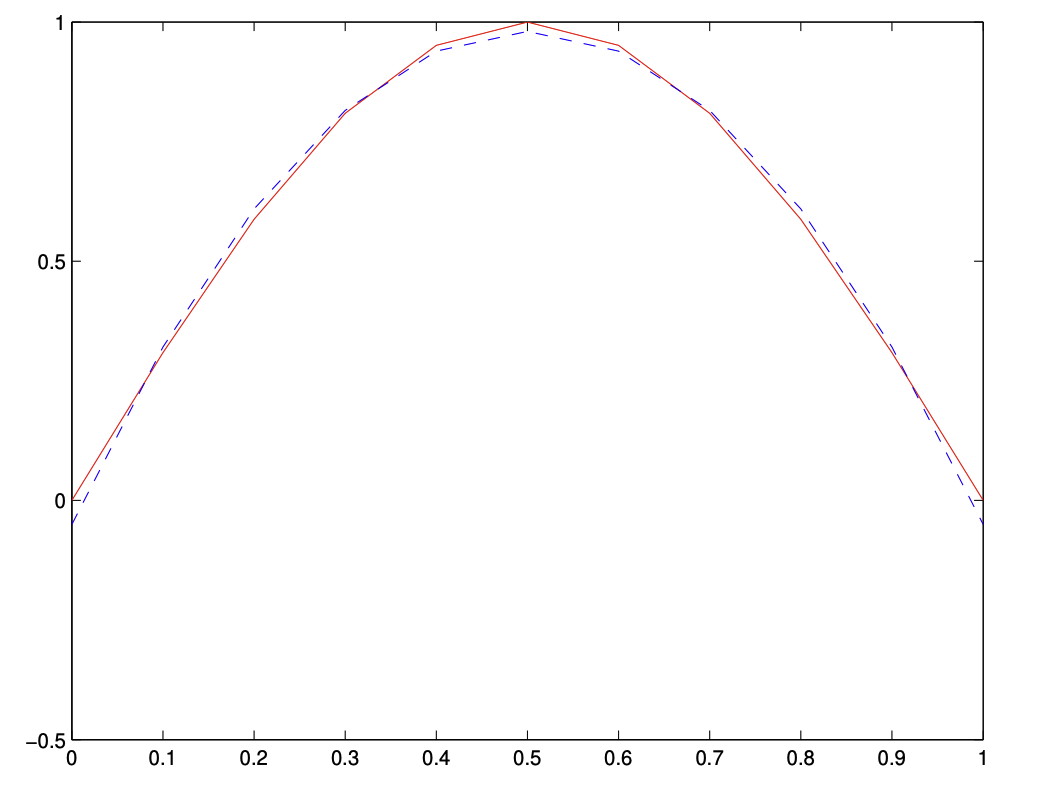
\includegraphics[width=0.5\textwidth]{Figures/appsin.png}
    \caption{Approximation of $\sin (\pi x)$ by a degree $2$ polynomial}
\end{figure}

However, solving a $(n+1) \times (n+1)$ linear system is very time-consuming.

\subsection{Linearly Independent Functions}

\begin{definition}[Linearly independent functions]
    Functions $\{\phi_0, \phi_1, \cdots, \phi_n\}$ are linearly independent on $[a,b]$ if, whenever \[
        c_0 \phi_0(x) + c_1 \phi_1(x) + \cdots + c_n \phi_n(x) = 0, \quad \forall x \in [a,b]
    \]
    we have $c_0 = c_1 = \cdots = c_n = 0$.
\end{definition}

\begin{theorem}
    For linearly independent set of polynomials. If \begin{center}
        $\phi_j$ is a polynomial of degree $j$,
    \end{center}
    then \begin{center}
        $\{\phi_0, \phi_1, \cdots, \phi_n\}$ are linearly independent on $[a,b]$.
    \end{center}
\end{theorem}

\begin{proposition}
    Any polynomial of degree $\leq n$, can be written uniquely as a linear combination of $\{\phi_0, \phi_1, \cdots, \phi_n\}$.
\end{proposition}

If $\{\phi_0, \phi_1, \cdots, \phi_n\}$ are linearly independent, and \[
    p_n(x) = \sum_{k=0}^n a_k \phi_k(x)
\]
then \[
    \min_{a_0, a_1, \cdots, a_n} E = \int_a^b \left(f(x) - \sum_{k=0}^n a_k \phi_k(x)\right)^2 \de x
\]
lead to \[
    0 = - \frac{\partial E}{\partial a_j} = 2 \int_a^b \left(f(x) - \sum_{k=0}^n a_k \phi_k(x)\right) \phi_j(x) \de x
\]

For $j=0,1,\dots,n$, we have \begin{equation}
    \sum_{k=0}^n a_k \int_a^b \phi_k(x) \phi_j(x) \de x = \int_a^b f(x) \phi_j(x) \de x \label{eq:7.1}
\end{equation}

\begin{definition}
    If $\{\phi_0, \phi_1, \cdots, \phi_n\}$ are chosen so that \[
        \int_a^b \phi_k(x) \phi_j(x) \de x = \begin{cases}
            0, & \mbox{if } j \neq k\\
            \alpha_k > 0, & \mbox{if } j = k
        \end{cases}
    \]
    we say they are \red{orthogonal} on $[a,b]$.
\end{definition}

If $\alpha_k = 1$ for $k=0,1,\dots,n$, we say they are \red{orthonormal} on $[a,b]$.
\begin{note}
    The reason $\alpha_k$ has to be positive is \[
        \int_a^b \phi_k(x)^2 \de x > 0
    \]
\end{note}

The eqs.~\ref{eq:7.1} becomes \[
    a_j \alpha_j = \int_a^b f(x) \phi_j(x) \de x
\]
i.e., \[
    a_j = \frac{1}{\alpha_j} \int_a^b f(x) \phi_j(x) \de x
\]
which is a simple formula with only one variable $a_j$ to solve.

\subsection{Trigonometric Polynomials Approximation}

\begin{theorem}
    Consider $\{\phi_0, \phi_1, \cdots, \phi_{2n-1}\}$ such that \[
        \phi_0(x) = \frac{1}{2}
    \]
    \[
        \phi_k(x) = \cos kx, \quad k=1,2,\dots,n
    \]
    \[
        \phi_{n+k}(x) = \sin kx, \quad k=1,2,\dots,n-1
    \]
    is \red{orthogonal on $[-\pi, \pi]$}.
\end{theorem}
\begin{proof}
    If $k \neq j$, $k \in \{1,2,\dots,n\}$, $j \in \{1,2,\dots,n\}$, we have \[
        \int_{-\pi}^\pi \phi_{n+k}(x) \phi_{j}(x) \de x = \int_{-\pi}^\pi \sin kx \cos jx \de x
    \]
    Using \[
        \sin kx \cos jx = \frac{1}{2} (\sin (k+j)x + \sin (k-j)x)
    \]
    Plug in
    \begin{align*}
        \int_{-\pi}^\pi \phi_{n+k}(x) \phi_{j}(x) \de x &= \frac{1}{2} \int_{-\pi}^\pi (\sin (k+j)x + \sin (k-j)x) \de x \\
        &= \frac{1}{2} \left( \frac{-\cos (k+j)x}{k+j} + \frac{-\cos (k-j)x}{k-j} \right) \bigg\vert_{-\pi}^\pi = 0
    \end{align*}
    
    If $k = j$, \begin{align*}
        \int_{-\pi}^\pi \sin kx \cos kx \de x & = \frac{1}{2} \int_{-\pi}^\pi (\sin 2kx) \de x \\
        &= \frac{-1}{4k} \cos 2kx \bigg\vert_{-\pi}^\pi = 0
    \end{align*}
    
    There are two other cases:
    \begin{itemize}
        \item $k, j$, $k = 1, 2, \dots, n$, $j = 1, 2, \dots, n$
        \item $n + k, n + j$, $k = 1, 2, \dots, n-1$, $j = 1, 2, \dots, n-1$
    \end{itemize}

    \begin{note}
        Some derivations include $\sin nx$ as well, though it is not necessary for the approximation.
    \end{note}

    Also we need to check $k = 0$. But they are all zero. Hence, we have shown that $\{\phi_0, \phi_1, \cdots, \phi_{2n-1}\}$ are orthogonal on $[-\pi, \pi]$.
\end{proof}

\vspace{1em}

Let \[
    S_n(x) = \frac{a_0}{2} + a_n \cos nx + \sum_{k=1}^{n-1} (a_k \cos kx + b_k \sin kx)
\]

With the orthalogonality, we have \begin{equation}
    a_k = \frac{\int_{-\pi}^\pi f(x) \cos kx \de x}{\int_{-\pi}^\pi \cos^2 kx \de x} = \frac{1}{\pi} \int_{-\pi}^\pi f(x) \cos kx \de x, \quad k=0,1,\dots,n \label{eq:7.2}
\end{equation}
\begin{equation*}
    b_k = \frac{\int_{-\pi}^\pi f(x) \sin kx \de x}{\int_{-\pi}^\pi \sin^2 kx \de x} = \frac{1}{\pi} \int_{-\pi}^\pi f(x) \sin kx \de x, \quad k=1,2,\dots,n-1
\end{equation*}

For the denominators, we can easily check that \[
    \int_{-\pi}^\pi \cos^2 kx \de x = \int_{-\pi}^\pi \sin^2 kx \de x = \pi
\]

\begin{note}
    The reason we use $\frac{a_0}{2}$ is that \[
        a_0 = \frac{\int_{-\pi}^\pi f(x) \frac{1}{2} \de x}{\int_{-\pi}^\pi \left(\frac{1}{2}\right)^2 \de x} = \frac{1}{\pi} \int_{-\pi}^\pi f(x) \de x = \frac{1}{\pi} \int_{-\pi}^\pi f(x) \cos 0 \cdot x \de x
    \]
    Then, it becomes consistent with eqs.~\ref{eq:7.2}.
\end{note}

\begin{remark}
    Why considering $\cos kx$ as well as $\sin kx$? But not $\cos kx$ alone? Because for the convergence theorem of Fourier series, we need to consider both $\cos kx$ and $\sin kx$.
\end{remark}

\subsection{Fourier Series}

The function we consider is
\[
    S_n(x) = \frac{a_0}{2} + a_n \cos nx + \sum_{k=1}^{n-1} (a_k \cos kx + b_k \sin kx)
\]
When $n \to \infty$, we have \[
    \lim_{n \to \infty} S_n(x)
\]
is called the ``Fourier series'' of $f(x)$. Under some conditions, we can show that \[
    S_n(x) \to f(x), \quad \mbox{as } n \to \infty
\]

Consider \[
    f(x) = |x| \quad \forall x \in (-\pi, \pi)
\]
\[
    a_0 = \frac{1}{\pi} \int_{-\pi}^\pi |x| \de x = \frac{2}{\pi} \int_0^\pi x \de x = \pi
\]
\begin{equation}
    a_k = \frac{1}{\pi} \int_{-\pi}^\pi |x| \cos kx \de x = \frac{2}{\pi} \int_0^\pi x \cos kx \de x \label{eq:7.3}
\end{equation}

Then \begin{align*}
    \int_0^\pi x \cos kx \de x &= x \frac{\sin kx}{k} \bigg\vert_0^\pi - \int_0^\pi \frac{\sin kx}{k} \de x \\
    &= \frac{\pi \sin k\pi}{k} + \frac{\cos kx}{k^2} \bigg\vert_0^\pi = \frac{(-1)^k - 1}{k^2}
\end{align*}

Therefore, from eq.~\ref{eq:7.3}, we have \[
    a_k = \frac{2}{\pi k^2} ((-1)^k - 1), \quad \forall k=1,2,\dots
\]

Because \[
    \sin x = -\sin (-x)
\]
we have \[
    |x| \sin x = - |-x| \sin (-x)
\]
and therefore \[
    b_k = \frac{1}{\pi} \int_{-\pi}^\pi |x| \sin kx \de x = 0, \quad \forall k=1,2,\dots
\]

Finally, \[
    S_n(x) = \frac{\pi}{2} + \frac{2}{\pi} \sum_{k=1}^n \frac{(-1)^k - 1}{k^2} \cos kx
\]
We can see \begin{equation*}
\begin{split}
    & S_0(x) = \frac{\pi}{2}, \text{ a straight line}\\
    & S_1(x) = \frac{\pi}{2} - \frac{4}{\pi}
    \cos x \\
    & S_2(x) = \frac{\pi}{2} - \frac{4}{\pi}
    \cos x + 0 \\
    & S_3(x) = \frac{\pi}{2} - \frac{4}{\pi}
    \cos x - \frac{4}{9\pi} \cos 3x 
\end{split}
\end{equation*}

\begin{note}
    This example we only use $\cos kx$ because $b_k = 0$ for all $k$. In general, we need to use both $\cos kx$ and $\sin kx$ to approximate a function.
\end{note}